\documentclass[12pt]{article}
\usepackage{amsmath,amssymb}
\usepackage{graphicx}
\usepackage{multirow}
\usepackage[usenames,dvipsnames]{xcolor}
\usepackage[utf8]{inputenc}
\usepackage[spanish,es-tabla]{babel}

\begin{document}

\title{TALLER 1}
\author{Miguel Angel Castillo Espitia}
\date{Febrero, 2019}
\maketitle


\section{Teoría}

Cuando un cuerpo se desplaza cerca de la superficie de la tierra, experimenta el campo gravitacional de esta como una fuerza constante. Dado que no se le ejercen más fuerzas a su trayectoria, podemos definir su trayectoria en un marco de coordenadas que llamaremos (x,y). Las ecuaciones de movimiento en este marco de coordenadas son las siguientes:\



\begin{equation}
  \begin{aligned}
	  {x(t)}={x}_{0}+{v}_{x0}{t}
	  \label{eq1}
  \end{aligned}
\end{equation}

\begin{equation}
  \begin{gathered}
	  {y(t)}={y}_{0}+{v}_{y0}{t}-\frac{g}{2}{t^{2}}
	  \label{eq2}
  \end{gathered}
\end{equation}

Dado que nosotros en nuestro experimento solo dejaremos caer un objeto verticalmente, sin ejercerle ninguna fuerza en el eje horizontal, para este experimento solo necesitaríamos la ecuación (\ref{eq2}). Luego de esta ecuacion podemos despejar la constante $\textstyle{g}$  y así obtener su valor.

\section{Experimento}

El experimento se basa en capturar un video donde se muestre la caída de un objeto de color sólido. Primero, elegimos el trasfondo donde tomaremos el video. Despues, ubicamos la cámara a un ángulo de 90 grados con respecto al movimiento del objeto. Cuando la cámara esté centrada en el trasfondo, procedemos a colocar dos marcas de color sólido separadas por un metro, esto con el fin de hallar un factor de conversión de las unidades de distancia de la imágen(pixeles) a metros. Luego grabamos la caída del objeto.
Luego para la recolección y el almacenamiento de los datos, usaremos el programa \sffamily{detection.py}, \rmfamily que nos retornará los datos sobre la trayectoria del objeto. Luego pasamos a analizar los datos y a detectar solo los datos relevantes (esto dado que el programa puede que detecte datos sobre otros objetos en el video). Despues de esto, obtenemos, gracias a las marcas que pusimos en un principio, los factores de conversión. Luego, podemos hacer una regresión cuadrática basándonos en la ecuación \ref{eq2}, para así obtener el valor   de $\textstyle{g}$. 

Después, hacemos el mismo procedimiento con más videos, con el fin de hallar el valor promedio de $\textstyle{g}$ y así obtener el error de la g calculada y la desviación estándar de las mediciones de la constante.

Luego de realizar el experimento, obtenemos que la desviación promedio es igual a **** y el valor promedio de $\textstyle{g}$ 

En la siguiente gráfica se muestra a g, representada como una funcion de la posición respecto al tiempo.
\begin{figure}[h]
	\centering
	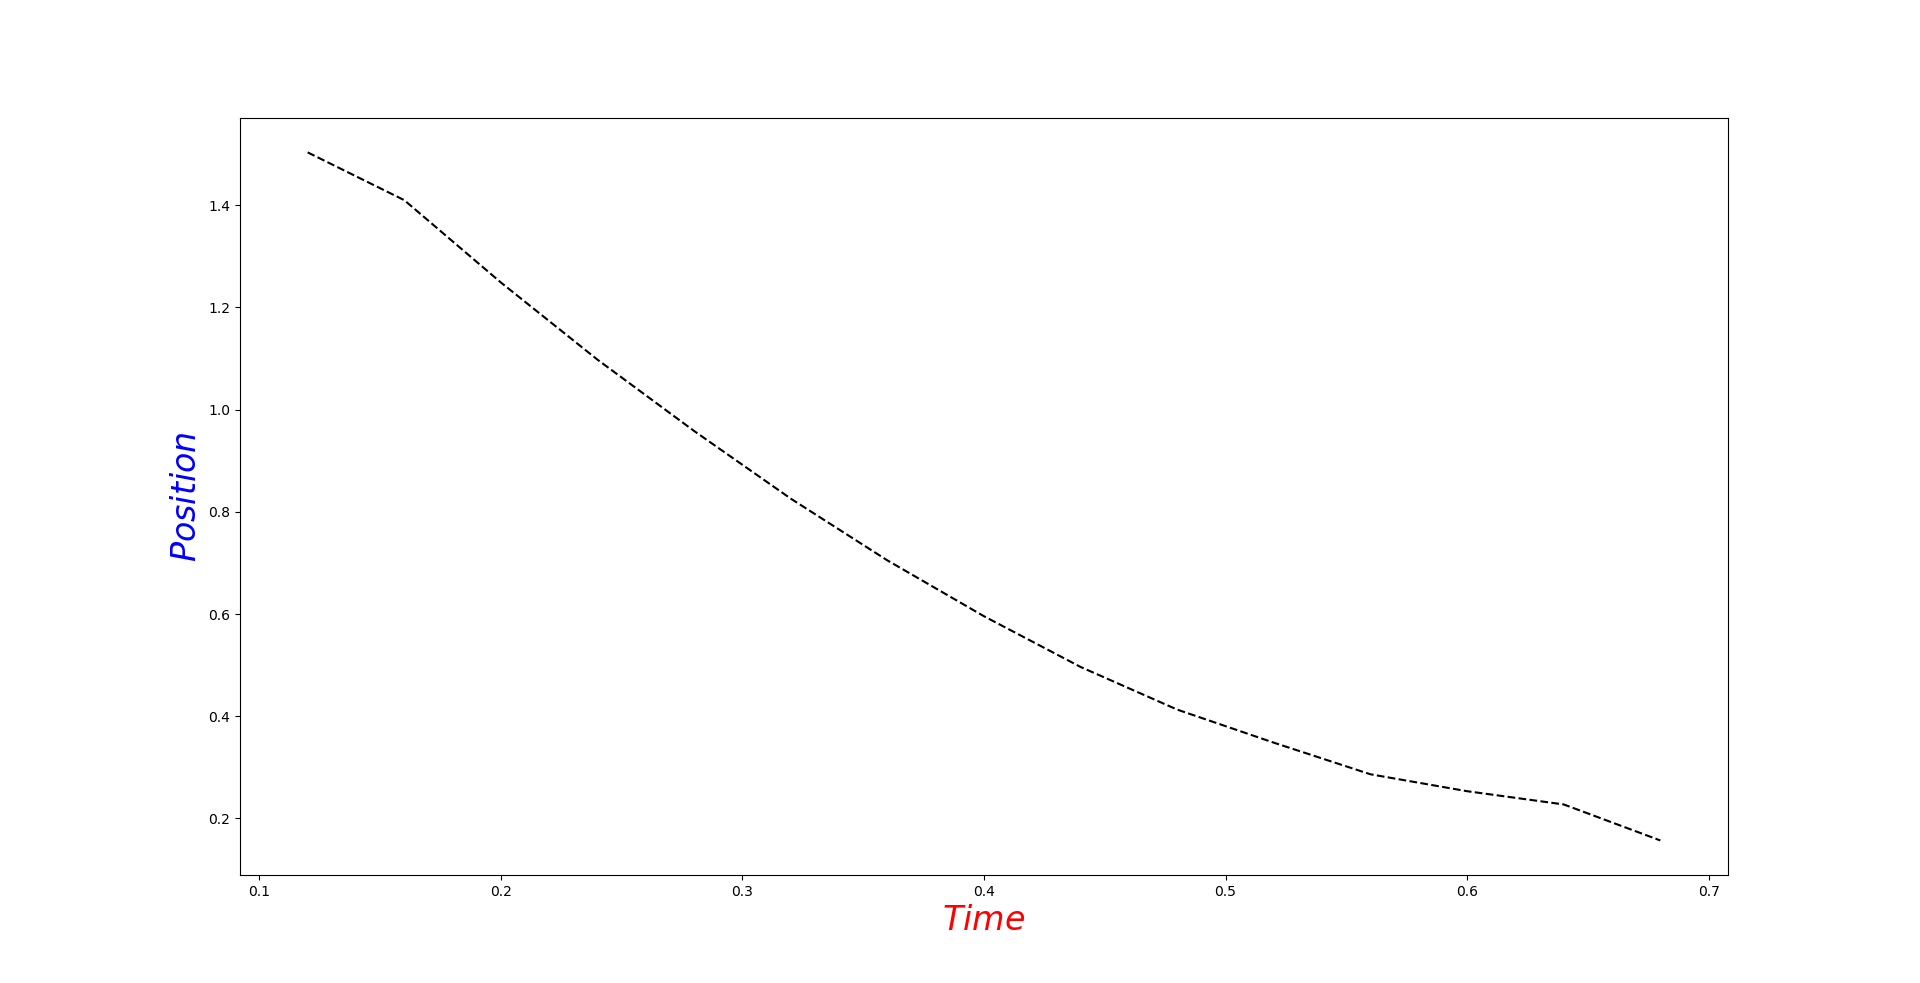
\includegraphics[scale=0.8]{Grafica.png}
	\caption{Grafica de la constante g}
	\label{graph1}
\end{figure}
\\







La siguiente tabla muestra los datos obtenidos de la realización del experimento:

\begin{table}[h]
	\centering
	\begin{tabular}{|c|c|c|c|}
		\hline
		tiempo($s$) & posición($m$) & velocidad$(m/s)$ & aceleración$(m/s^{2})$ \\
		\hline\hline
		0 & dato & 0 & dato \\
		\hline
		dato & dato & dato & dato \\
		\hline
		dato & dato & dato & dato \\
		\hline
		dato & dato & dato & dato \\
		\hline
		dato & dato & dato & dato \\
		\hline
		dato & dato & dato & dato \\
		\hline
		dato & dato & dato & dato \\
		\hline
		dato & dato & dato & dato \\
		\hline
		dato & dato & dato & dato \\
		\hline
	\end{tabular}
	\caption{}
	\label{table1}
\end{table}


\section{Análisis}

Con la ecuación:\\
\begin{equation}
	\begin{aligned}
		{g}=\frac{G{M}_{e}}{{{R}_{e}}^{2}}
		\label{eq3}
	\end{aligned}
\end{equation}\\

obtenemos que g es igual a **** y en nuestro experimento obtuvimos un valor promedio de g igual a ****. Podemos concluir que el valor medido es muy cercano al valor estimado, casi igual. La diferencia de valores podría ser causada gracias a:\\
-Una posible mala selección de datos.\\
-Mal calculo de factores de conversión.\\
-Mala ambientación para la toma del video.\\
-Posible recopilación de datos irrelevantes.\\

\\
\\

\begin{thebibliography}{}

\bibitem{milibro}
  D. Kleppner and R. Kolenkow, {\it An introduction to mechanics 2ed,} Cambridge University Presss (2014)

\bibitem{Proesmans}
  H.D. Young, R.A. Freedman and Addison-Wesley, {\it University Physics (13 ed.,} Addison-Wesley  (2012)
    
\end{thebibliography}

\end{document}